\documentclass{article}
\usepackage[utf8]{inputenc}
\usepackage[left=3cm, right=3cm, top=2cm]{geometry}
\title{Stability conditions and von Neumann Analysis}
\author{Silvin Willemsen}
\date{March 2019}
\usepackage{natbib}
\usepackage{graphicx}
\usepackage{appendix}
\usepackage{amsmath}
\usepackage{amsfonts}
\usepackage{amssymb}

\begin{document}

\maketitle

\section{Introduction}
In this document I will show the calculations for different von Neumann analyses and stability conditions.

% \begin{figure}[h!]
% \centering
% 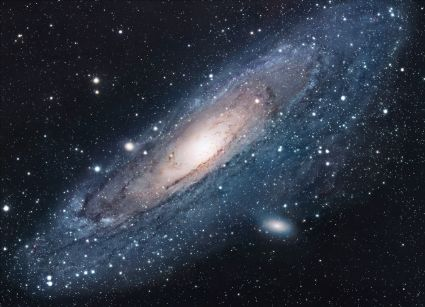
\includegraphics[scale=1.7]{universe}
% \caption{The Universe}
% \label{fig:universe}
% \end{figure}
\section{Identities}

\begin{equation}\label{eq:sinIdentity}
    \sin(x) = \frac{e^{jx} - e^{-jx}}{2j}\quad \Longrightarrow \quad \sin^2(x) = \frac{e^{j2x} - 2e^{jx-jx}+ e^{-j2x}}{-4} = \frac{e^{j2x} + e^{-j2x}}{-4} + \frac{1}{2}.
\end{equation}
From this we can derive the useful identity for $\sin^4(x)$:

\begin{align}
    \sin^4(x) = (\sin^2(x))^2 &= \Bigg(\frac{e^{j2x} + e^{-j2x}}{-4} + \frac{1}{2}\Bigg)^2\nonumber\\
    &=\Bigg(\frac{e^{j2x} + e^{-j2x}}{-4}\Bigg)^2 + \frac{e^{j2x} + e^{-j2x}}{-4} + \frac{1}{4}\nonumber\\
    &=\frac{e^{j4x} + e^{-j4x}}{16} + \frac{1}{8} + \underbrace{\frac{e^{j2x} + e^{-j2x}}{-4}}_\text{$\sin^2(x)- \frac{1}{2}$} + \frac{1}{4}\nonumber\\
    &= -\frac{1}{4}\Bigg(\frac{e^{j4x} + e^{-j4x}}{-4} + \frac{1}{2}\Bigg) + \frac{2}{8} + \sin^2(x) - \frac{1}{2} + \frac{1}{4}\nonumber\\
    &= -\frac{1}{4}\sin^2(2x) + \sin^2(x) \label{eq:sin4}
\end{align}
\subsection{Frequency domain analysis}
See section 5.2.6 of \cite{Bilbao2009}:
\begin{equation}
    u_l^n = z^n e^{jl\beta h}
\end{equation}
where $\beta$ is a real wavenumber. Important to remember is that without a shift in space (fx. $l+1$) or time (fx. $n-1$) $l = 0$ or $n=0$ respectively:
\begin{subequations} \label{eq:identitiesZ}
    \begin{align}
        u_l^n &= z^0 e^{j0\beta h} = 1\\
        u_{l+1}^n &= z^0 e^{j1\beta h} = e^{j\beta h}\\
        u_{l-1}^n &= z^0 e^{j(-1)\beta h} = e^{-j\beta h}\\
        u_{l+2}^n &= z^0 e^{j2\beta h} = e^{j\beta h}\\
        u_{l-2}^n &= z^0 e^{j(-2)\beta h}= e^{-j2\beta h}\\
        u_l^{n+1}&= z^1 e^{j0\beta h} = z\\
        u_l^{n-1}&= z^{-1} e^{j0\beta h} = z^{-1}
    \end{align}
\end{subequations}

\section{1D Wave Equation}
This section will derive the stability condition for the 1D wave equation. Starting from the FDS (Eq. 6.35)
\begin{equation}
    u_l^{n+1} = 2(1-\lambda^2)u_l^n + \lambda^2(u_{l+1}^n+u_{l-1}^n)-u_l^{n-1},
\end{equation}
where
\begin{equation}\label{eq:lambda}
    \lambda = \frac{ck}{h} \quad \text{and wave speed} \quad c = \sqrt{\frac{T}{\rho A}},
\end{equation}
with tension $T$, material density $\rho$ and cross-sectional area $A$.
We can now perform frequency domain analysis. Moving all terms to the left of the equals-sign and with their respective identities found in Eqs. \eqref{eq:identitiesZ} filled in, we get:
\begin{equation}\label{eq:zFDS}
    z - 2(1-\lambda^2)1 - \lambda^2(e^{j\beta h}+e^{-j\beta h}) + z^{-1} = 0.
\end{equation}
Using the identity found in Eq. \eqref{eq:sinIdentity} with $\beta h = 2x \Rightarrow x = \beta h / 2$ we can rewrite \eqref{eq:zFDS} to:
\begin{equation}
     z - 2 + 2\lambda^2 +4\lambda^2(\sin^2({\beta h / 2}) - 1/2) - z^{-1} = 0,
\end{equation}
and rewriting this yields the characterstic equation shown in Eq. (6.38):
\begin{equation}\label{eq:characteristic1D}
     z + 2(2\lambda^2\sin^2(\beta h/2) - 1) + z^{-1} = 0.
\end{equation}
The roots are then given by (using $X = \lambda^2\sin^2(\beta h/2)$):
\begin{equation}
\begin{aligned}\nonumber
    z_\pm &= \frac{-2(2X-1) \pm \sqrt{4(2X-1)^2 - 4 \cdot 1 \cdot 1}}{2}\\
    &= 1-2X \pm 1/2 \cdot \sqrt{4(2X-1)^2 - 4}\\
    &= 1-2X \pm 1/2 \cdot \sqrt{4(4X^2-4X + 1) - 4}\\
    &= 1-2X \pm 1/2 \cdot \sqrt{(4(4X^2 - 4X) + 4 - 4}\\
    &= 1-2X \pm 1/2 \cdot \sqrt{4(4X^2 - 4X)}\\
    &= 1-2X \pm 1/2 \cdot 2 \cdot \sqrt{4X^2 - 4X}\\
    &= 1-2X \pm \sqrt{(1 - 2X)^2 - 1}\\
\end{aligned}
\end{equation}
which results in the equation for the roots (right below (6.38) in section 6.2.2):
\begin{equation}
    z_\pm = 1-2\lambda^2\sin^2(\beta h/2) \pm \sqrt{(1 - 2\lambda^2\sin^2(\beta h/2))^2 - 1}.
\end{equation}
The scheme is then stable when these roots are bounded by unity for all $\beta$ \cite{BilbaoTutorial2018}
\begin{equation}\label{eq:boundByUnity}
    |z| \leq 1.
\end{equation} 
It can be shown that for a polynomial of the form 
\begin{equation}\label{eq:polynomialForm}
    z^2 + a^{(1)}z + a^{(2)}
\end{equation} it follows condition \eqref{eq:boundByUnity} when it abides the following (Eq. 2.14)
\begin{equation}\label{eq:condition214}
    |a^{(1)}| - 1 \leq a^{(2)} \leq 1,
\end{equation}
and when applied to the characteristic equation \eqref{eq:characteristic1D} (after multiplication with $z$), it can be seen that
\begin{equation}\nonumber
    \begin{aligned}
        |2(2\lambda^2\sin^2(\beta h/2) - 1)|-1 &\leq 1\\
        |2(2\lambda^2\sin^2(\beta h/2) - 1)| &\leq 2\\
        |2\lambda^2\sin^2(\beta h/2) - 1| &\leq 1,
    \end{aligned}    
\end{equation}
which is the equation right above Eq. (6.39). This can then be rewritten as
\begin{equation}\nonumber
    \begin{aligned}
        -1 \leq 2\lambda^2\sin^2(\beta h/2) - 1 &\leq 1\\
        0 \leq 2\lambda^2\sin^2(\beta h/2)&\leq 2\\
        0\leq \lambda^2\sin^2(\beta h/2) &\leq 1
    \end{aligned}
\end{equation}
and observing that all terms are squared, the result will always be non-negative, yielding Eq. (6.39):
\begin{equation}
     \lambda^2\sin^2(\beta h/2) \leq 1.
\end{equation}
Furthermore, knowing that the $\sin^2(\beta h / 2)$-term is bounded by $1$ for all $\beta$ the following condition is sufficient for stability (Eq. 6.40):
\begin{equation}
    \lambda \leq 1.
\end{equation}
Recalling \eqref{eq:lambda}, we see that the grid spacing is bounded by the following condition:
\begin{equation}
    h \geq h_\text{min} = ck.
\end{equation}
The closer $h$ is to $h_\text{min}$, the higher the quality of the implementation. 
\section{Ideal Bar}
Starting with the update equation for the ideal bar (eq. 7.12):
\begin{equation}
    u_l^{n+1}=(2-6\mu^2)u_l^n+4\mu^2(u_{l+1}^n+u_{l-1}^n)-\mu^2(u_{l+2}^n+u_{l-2}^n)-u_l^{n-1},
\end{equation}
where 
\begin{equation}\label{eq:mu}
    \mu = \frac{\kappa k}{h^2} \quad \text{and} \quad \kappa = \sqrt{\frac{EI}{\rho A}},
\end{equation}
we can perform frequency domain analysis by filling in the identities from Eqs. \eqref{eq:identitiesZ} yielding
\begin{equation}\label{eq:zFDSBar}
    z-2+6\mu^2-4\mu^2(e^{j\beta h}+e^{-j\beta h}) + \mu^2 (e^{j2\beta h}+e^{-j2\beta h}) + z^{-1} = 0.
\end{equation}
Again, using the identity found in Eq. \eqref{eq:sinIdentity} with $\beta h = 2x \Rightarrow x = \beta h / 2$ we can rewrite \eqref{eq:zFDSBar} to

\begin{equation}\nonumber
    \begin{aligned}
        &z-2+6\mu^2+16\mu^2(\sin^2(\beta h / 2)) - 8\mu^2  -4 \mu^2 (\sin^2(\beta h)) + 2\mu^2 + z^{-1} = 0\\
        &z-2+16\mu^2(\sin^2(\beta h / 2)) -4 \mu^2 (\sin^2(\beta h)) + z^{-1} = 0.
    \end{aligned}  
\end{equation}
We can rewrite the above to
\begin{equation}\nonumber
    z-2+16\mu^2\bigg(-\frac{1}{4}\sin^2(\beta h)+\sin^2(\beta h / 2)\bigg) + z^{-1} = 0,
\end{equation}
and using Eq. \eqref{eq:sin4} we can simplify this to the characteristic equation (Eq. (7.13))

\begin{equation}
    z+(16\mu^2\sin^4(\beta h/2) - 2) + z^{-1} = 0.
\end{equation}
The parentheses are used here to denote that $16\mu^2\sin^4(\beta h/2) - 2$ is a single term ($a^{(1)}$) in condition \eqref{eq:condition214}. Using this condition we get
\begin{equation}\nonumber
    \begin{aligned}
        |16\mu^2\sin^4(\beta h/2) - 2|-1&\leq 1\\
        |8\mu^2\sin^4(\beta h/2) - 1|&\leq 1\\
        -1\leq8\mu^2\sin^4(\beta h/2) - 1&\leq 1\\
        0\leq8\mu^2\sin^4(\beta h/2)&\leq 2\\
        0\leq\mu^2\sin^4(\beta h/2)&\leq \frac{1}{4},
    \end{aligned}
\end{equation}
and as the $\sin^4(\beta h/2)$-term is again bounded by 1 and observing that all terms are squared, so non-negative, we get Eq. (7.14)
\begin{equation}
    \mu^2 \leq \frac{1}{4}\quad \Longleftrightarrow\quad \mu \leq \frac{1}{2}.
\end{equation}
Recalling \eqref{eq:mu} we get the stability condition in terms of grid spacing $h$ 
    \begin{equation}
    \frac{\kappa k}{h^2}\leq \frac{1}{2}\quad \Longleftrightarrow\quad h \geq h_\text{min} = \sqrt{2\kappa k}.
\end{equation}

\section{Stiff String}
The characteristic equation for the stiff string, after obtaining the following update equation
\begin{equation}
    u_l^{n+1}=(2-2\lambda^2-6\mu^2)u_l^n+(\lambda^2+4\mu^2)(u_{l+1}^n+u_{l-1}^n)-\mu^2(u_{l+2}^n+u_{l-2}^n)-u_l^{n-1}
\end{equation}
can, after frequency domain analysis, be shown to be
\begin{equation}
    z + (4\lambda^2\sin^2(\beta h/2)+16\mu^2\sin^4(\beta h/2)-2) +z^{-1} = 0.
\end{equation}
Using \eqref{eq:condition214} and solving the inequality in terms of $\lambda$ and $\mu$ we get
\begin{equation}\nonumber
    \begin{aligned}
    |4\lambda^2\sin^2(\beta h/2)+16\mu^2\sin^4(\beta h/2)-2|-1&\leq 1\\
    0\leq\lambda^2\sin^2(\beta h/2)+4\mu^2\sin^4(\beta h/2)&\leq 1,
    \end{aligned}
\end{equation}
which, after observing the $\sin$-terms to be bounded by 1 and non-negativity of the solution through the squared terms, we obtain Eq. (7.24)
\begin{equation}
    \lambda^2+4\mu^2\leq 1.
\end{equation}
Recalling \eqref{eq:lambda} and \eqref{eq:mu}, solving for $h$ yields
\begin{equation}
    \begin{aligned}
        \frac{c^2k^2}{h^2} + 4 \frac{\kappa^2h^2}{h^4}\leq 1\\
        h^4 - c^2k^2h^2+4\kappa^2k^2 \geq 0,
    \end{aligned}
\end{equation}
and its minimum value can be found
\begin{equation}
    h \geq h_\text{min} = \sqrt{\frac{c^2k^2+\sqrt{c^4k^4-16\kappa^2k^2}}{2}}.
\end{equation}
\subsection{Adding Damping}
Adding damping to the stiff string will result in the following update equation:
\begin{equation}\label{eq:dampedStiffString}
    \begin{aligned}
    (1+\sigma_0k)u_l^{n+1} &= (2-2\lambda^2-6\mu^2-\frac{4\sigma_1k}{h^2})u_l^n +(\lambda^2 + 4\mu^2 + \frac{2\sigma_1k}{h^2})(u_{l+1}^n+u_{l-1}^n)\\
    &-\mu^2(u_{l+2}^n+u_{l-2}^n)+(-1 + \sigma_0k+\frac{4\sigma_1k}{h^2})u_l^{n-1} -\frac{2\sigma_1k}{h_2}(u_{l+1}^{n-1}+u_{l-1}^{n-1}),
    \end{aligned}
\end{equation}
where $\sigma_0 \geq 0$ and $\sigma_1\geq0$ are the frequency independent and frequency dependent damping respectively. The characteristic equation of \eqref{eq:dampedStiffString} can be shown to be
\begin{equation}
    (1+\sigma_0k)z + \bigg(16\mu^2\sin^4(\beta h/2)+(4\lambda^2+\frac{8\sigma_1k}{h^2})\sin^2(\beta h/2) - 2\bigg)+\bigg(1-\sigma_0k-\frac{8\sigma_1k}{h^2}\sin^2(\beta h/2)\bigg)z^{-1}=0.
\end{equation}
Dividing by $(1+\sigma_0k)$ to get a polynomial of the form presented in \eqref{eq:polynomialForm} and employing \eqref{eq:condition214} yields

\begin{equation}\nonumber
    \begin{aligned}
        &\Bigg|\frac{16\mu^2\sin^4(\beta h/2)+(4\lambda^2+\frac{8\sigma_1k}{h^2})\sin^2(\beta h/2) - 2}{1+\sigma_0k}\Bigg|-1 \leq \frac{1-\sigma_0k-\frac{8\sigma_1k}{h^2}\sin^2(\beta h/2)}{1+\sigma_0k}\leq 1\\
        &\Big|16\mu^2\sin^4(\beta h/2)+(4\lambda^2+\frac{8\sigma_1k}{h^2})\sin^2(\beta h/2) - 2\Big|\leq2-\frac{8\sigma_1k}{h^2}\sin^2(\beta h/2)\leq2+2\sigma_0k.
    \end{aligned}
\end{equation}
Assuming the lowest possible value for $\sigma_0$ (which is 0) and subtracting 2 from all, we get the following inequality
\begin{equation}
        \Big|16\mu^2\sin^4(\beta h/2)+(4\lambda^2+\frac{8\sigma_1k}{h^2})\sin^2(\beta h/2) - 2\Big|-2\leq-\frac{8\sigma_1k}{h^2}\sin^2(\beta h/2)\leq0.
\end{equation}
It can be concluded that the last inequality will be satisfied for any value of $\beta$, i.e. $-\frac{8\sigma_1k}{h^2}\sin^2(\beta h/2)$ will always be less or equal to zero. Removing this inequality and continuing the derivation gives
\begin{equation}
    0 \leq 16\mu^2\sin^4(\beta h/2) + 4\lambda^2\sin^2(\beta h/2) \leq 4-\frac{16\sigma_1k}{h^2}\sin^2(\beta h/2).
\end{equation}
Again, we know that the first inequality will always be satisfied (squared terms), so we can disregard this inequality as well. Continuing..
\begin{equation}
    \begin{aligned}
        4\mu^2\sin^4(\beta h/2) + \lambda^2\sin^2(\beta h/2)+\frac{4\sigma_1k}{h^2}\sin^2(\beta h/2) \leq 1.
    \end{aligned}
\end{equation}
Considering (again) the fact that the $\sin$-terms are bounded by 1 we get the condition
\begin{equation}
    4\mu^2 + \lambda^2 + \frac{4\sigma_1k}{h^2} \leq 1,
\end{equation}
which, again recalling \eqref{eq:lambda} and \eqref{eq:mu}, can be solved for $h$:
\begin{equation}
    \begin{aligned}
        &\frac{4\kappa^2k^2}{h^4}+\frac{c^2k^2-4\sigma_1k}{h^2} - 1 \leq 0,\\
        &h^4 - (c^2k^2-4\sigma_1k)h^2 - 4\kappa^2k^2 \geq 0,\\
        &h\geq\sqrt{\frac{c^2k^2+4\sigma_1k+\sqrt{(c^2k^2+4\sigma_1k)^2+16\kappa^2k^2}}{2}}
    \end{aligned}
\end{equation}
\bibliographystyle{plain}
\bibliography{references}
\end{document}
